\section{Counterfactual Error Analysis}
\label{sec:app_err_analysis}

%
\begin{figure}[t]
\centering
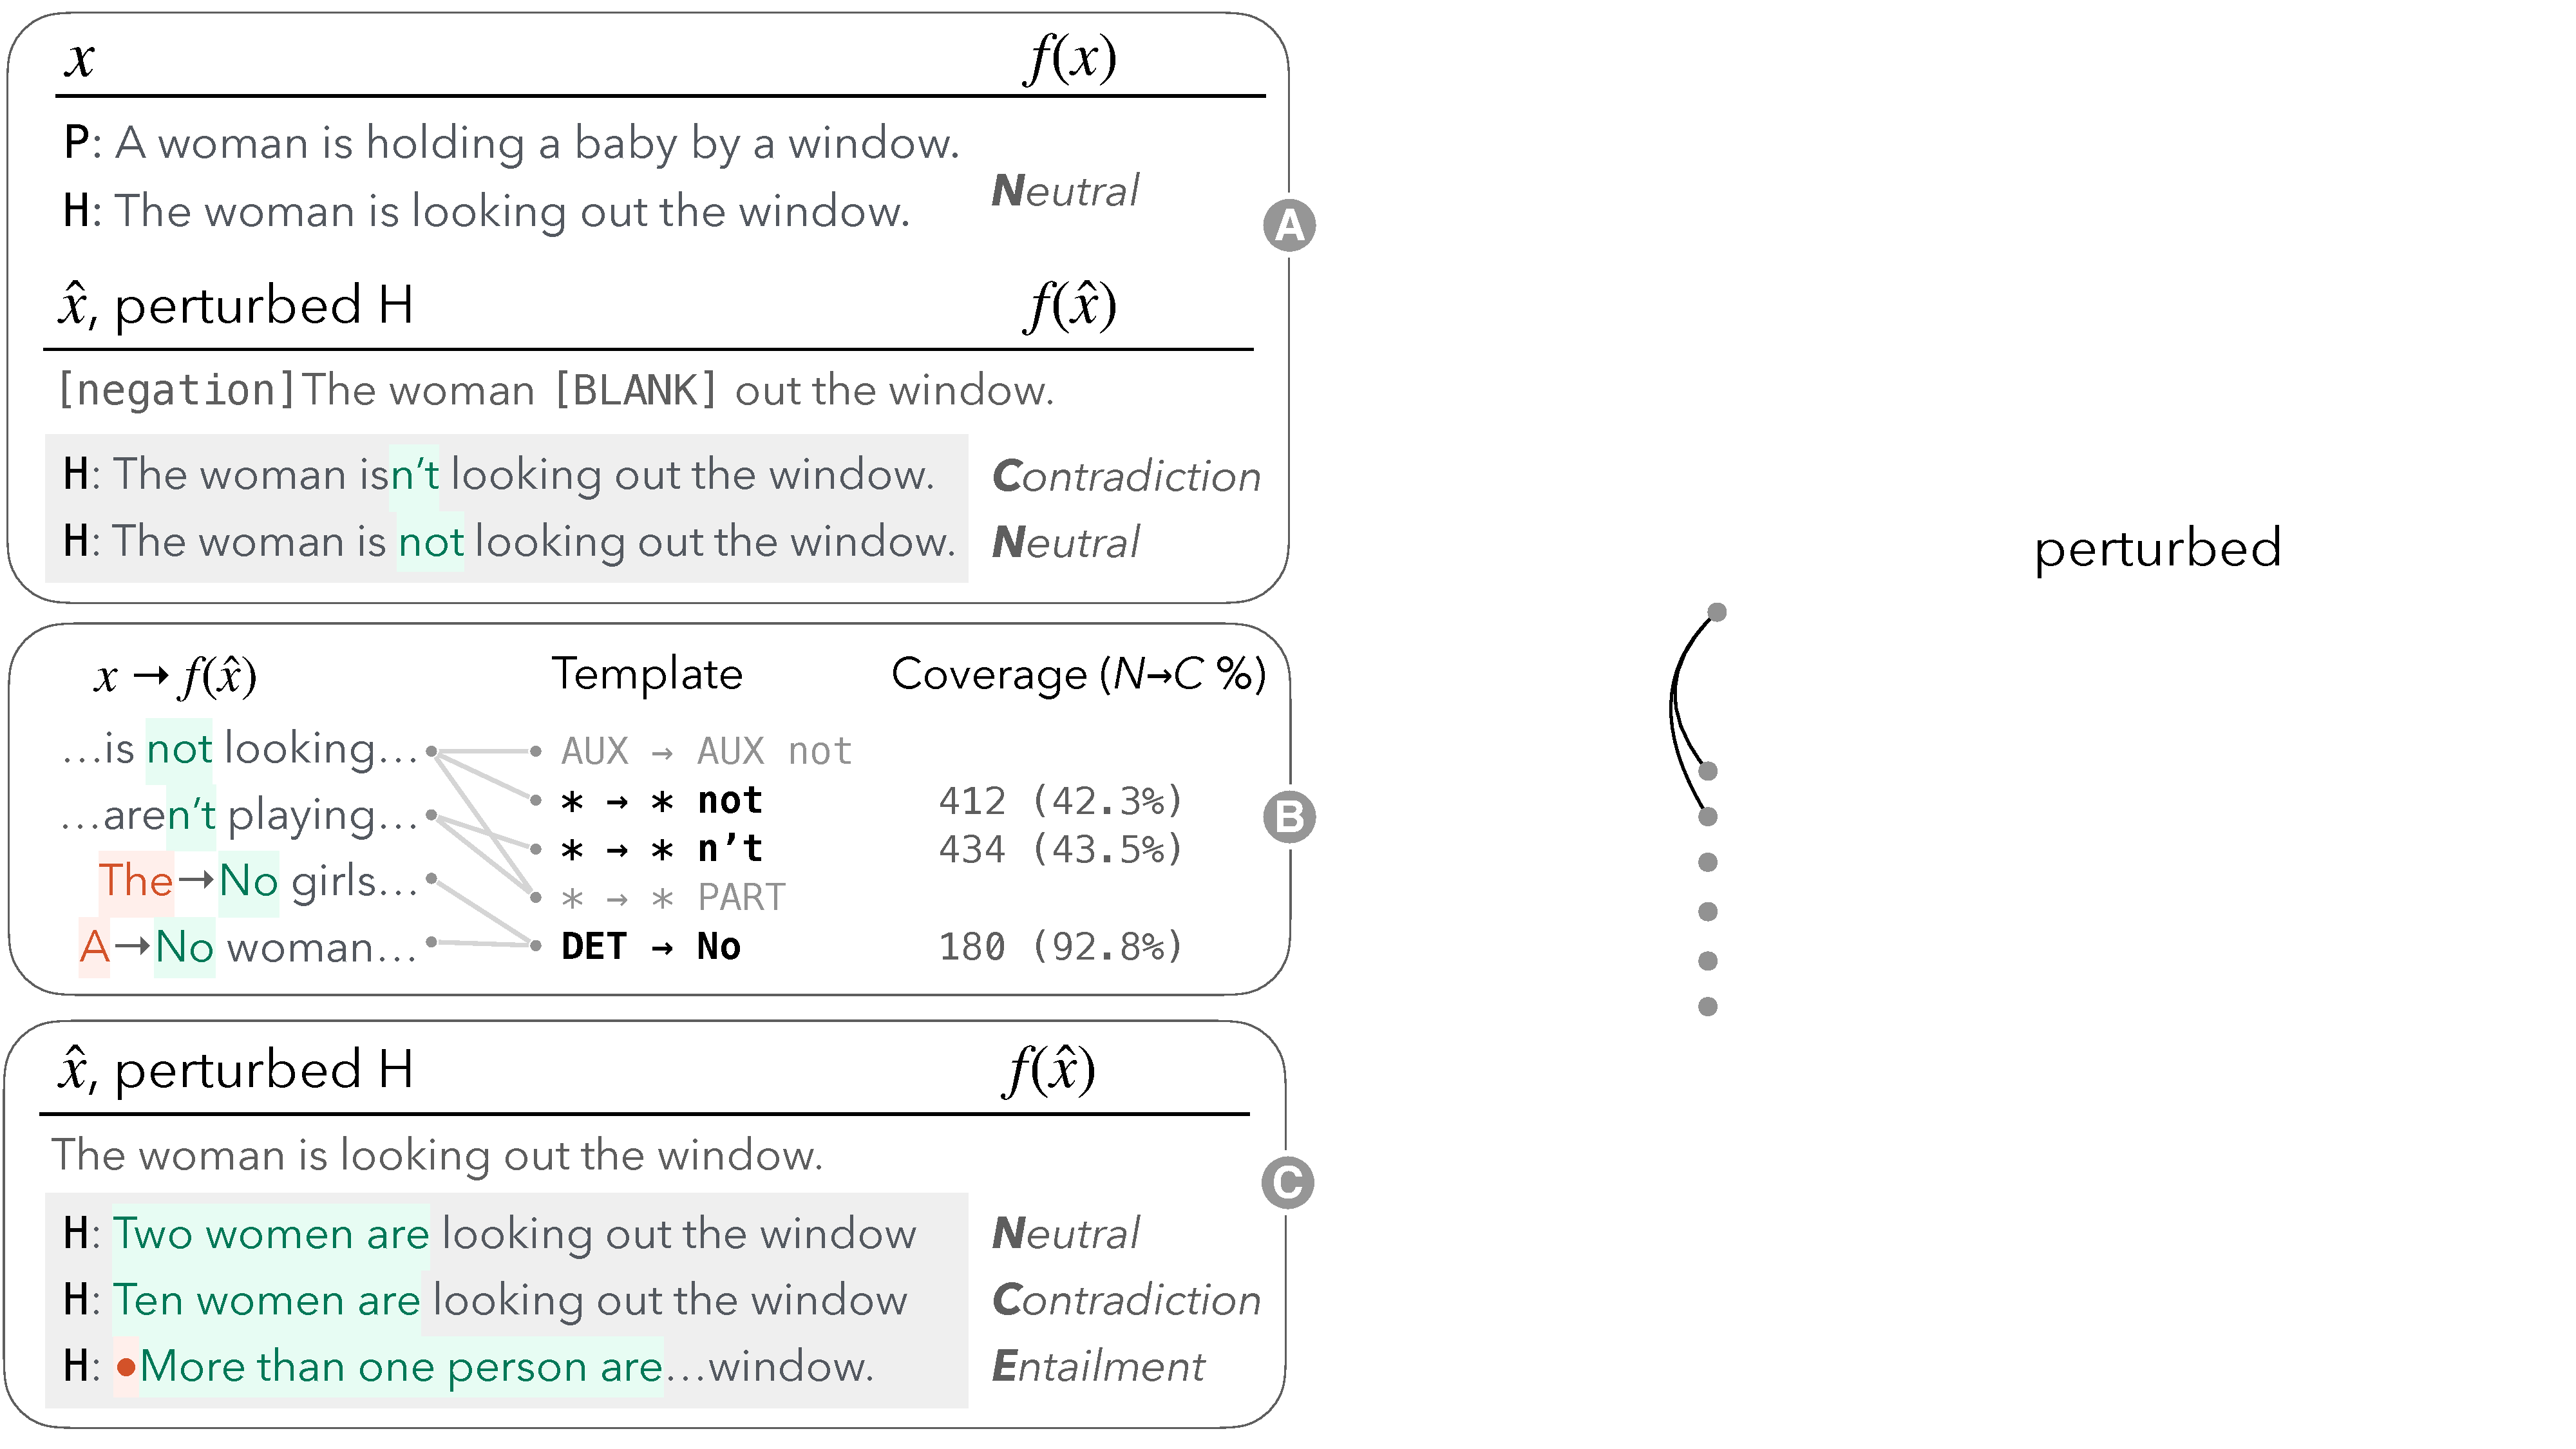
\includegraphics[trim={0 12.5cm 33cm 0cm},clip,width=1\columnwidth]{figures/err_analysis.pdf}
\vspace{-15pt}
\caption{
(A) An \nli case with a \emph{Neutral} prediction (the \uline{underlined} $f(\xp)$ are correct).
Through strict \tagstrs and blanks, \sysname generates two $\xp$ that negate the hypothesis sentence \emph{H}, which result in different predictions.
(B) Generalizing perturbation patterns beyond individual counterfactuals, we can systematically compare a model's response to different negations, \eg 92.8\% of the time the prediction flips from \emph{N}eutral~$\veryshortarrow$~\emph{C}ontradiction on \swap{\texttt{DET}}{no}.
%(C) Another blank placement that leads to analyses on \emph{quantifiers}.
}
\vspace{-10pt}
\label{fig:err_analysis}
\end{figure}


Previous applications focus on a selected subset of $\xp$, but access to the entire pool is also important.
Through a case study on the \nli RoBERTa model in \S\ref{subsec:contrast_set}, we demonstrate that \sysname's ability to generate \emph{multiple} counterfactuals per $x$ is essential for systematic error analysis~\cite{wu2019errudite}.
Here, the generation is largely driven by human analysts, and the relationship $\relation{\xp}$ can be determined by human domain expertise.

\emph{Form model behavior hypotheses by inspecting counterfactuals around one instance.}
\citet{gururangan2018annotation} asserted that negation is correlated with the class label \emph{contradiction}. 
To verify this, we can randomly select a \emph{neutral} instance $x$ as in Figure~\ref{fig:err_analysis}A, and inspect counterfactuals that \emph{only} negate the hypothesis sentence.
\sysname produces two $\xp$:
While \exinline{is\add{n't}} seems to confirm the overfit to negation, \exinline{is not} shows a counterexample. 
We therefore hypothesize that
\emph{the model has more nuanced responses to different kinds of negation}.
%, overfitting to some patterns more than others.

\emph{Verify the hypothesis through systematic counterfactual analysis.}
Does the observation generalize beyond one instance? 
We compare different negation patterns on \emph{a group of} 895 instances that have \emph{neutral} groundtruths and predictions.
For each $x$, we collect multiple counterfactuals by adding \ctrltag{negation} to the hypothesis, and extract \emph{negation templates} from each $\xp$ by abstracting the modified spans into linguistic features (as in Figure~\ref{fig:err_analysis}B).
Then, we select representative templates that cover various counterfactuals and are as concrete as possible. 
The method is similar to \citet{wu2020tempura}, and more details are in Appendix~\ref{appendix:err_analysis_template}.
The top three templates selected (in bold) show interesting contrasts:
First, counter to Figure~\ref{fig:err_analysis}A, the model is relatively stable on \add{not} and \add{n't} --- they both flip around 43\% \emph{neutral} predictions to \emph{contradiction}, while maintaining others.
However, the model does respond much more aggressively to \swap{\texttt{DET}}{no}, partially confirming our hypothesis.

\begin{figure}[t]
\centering
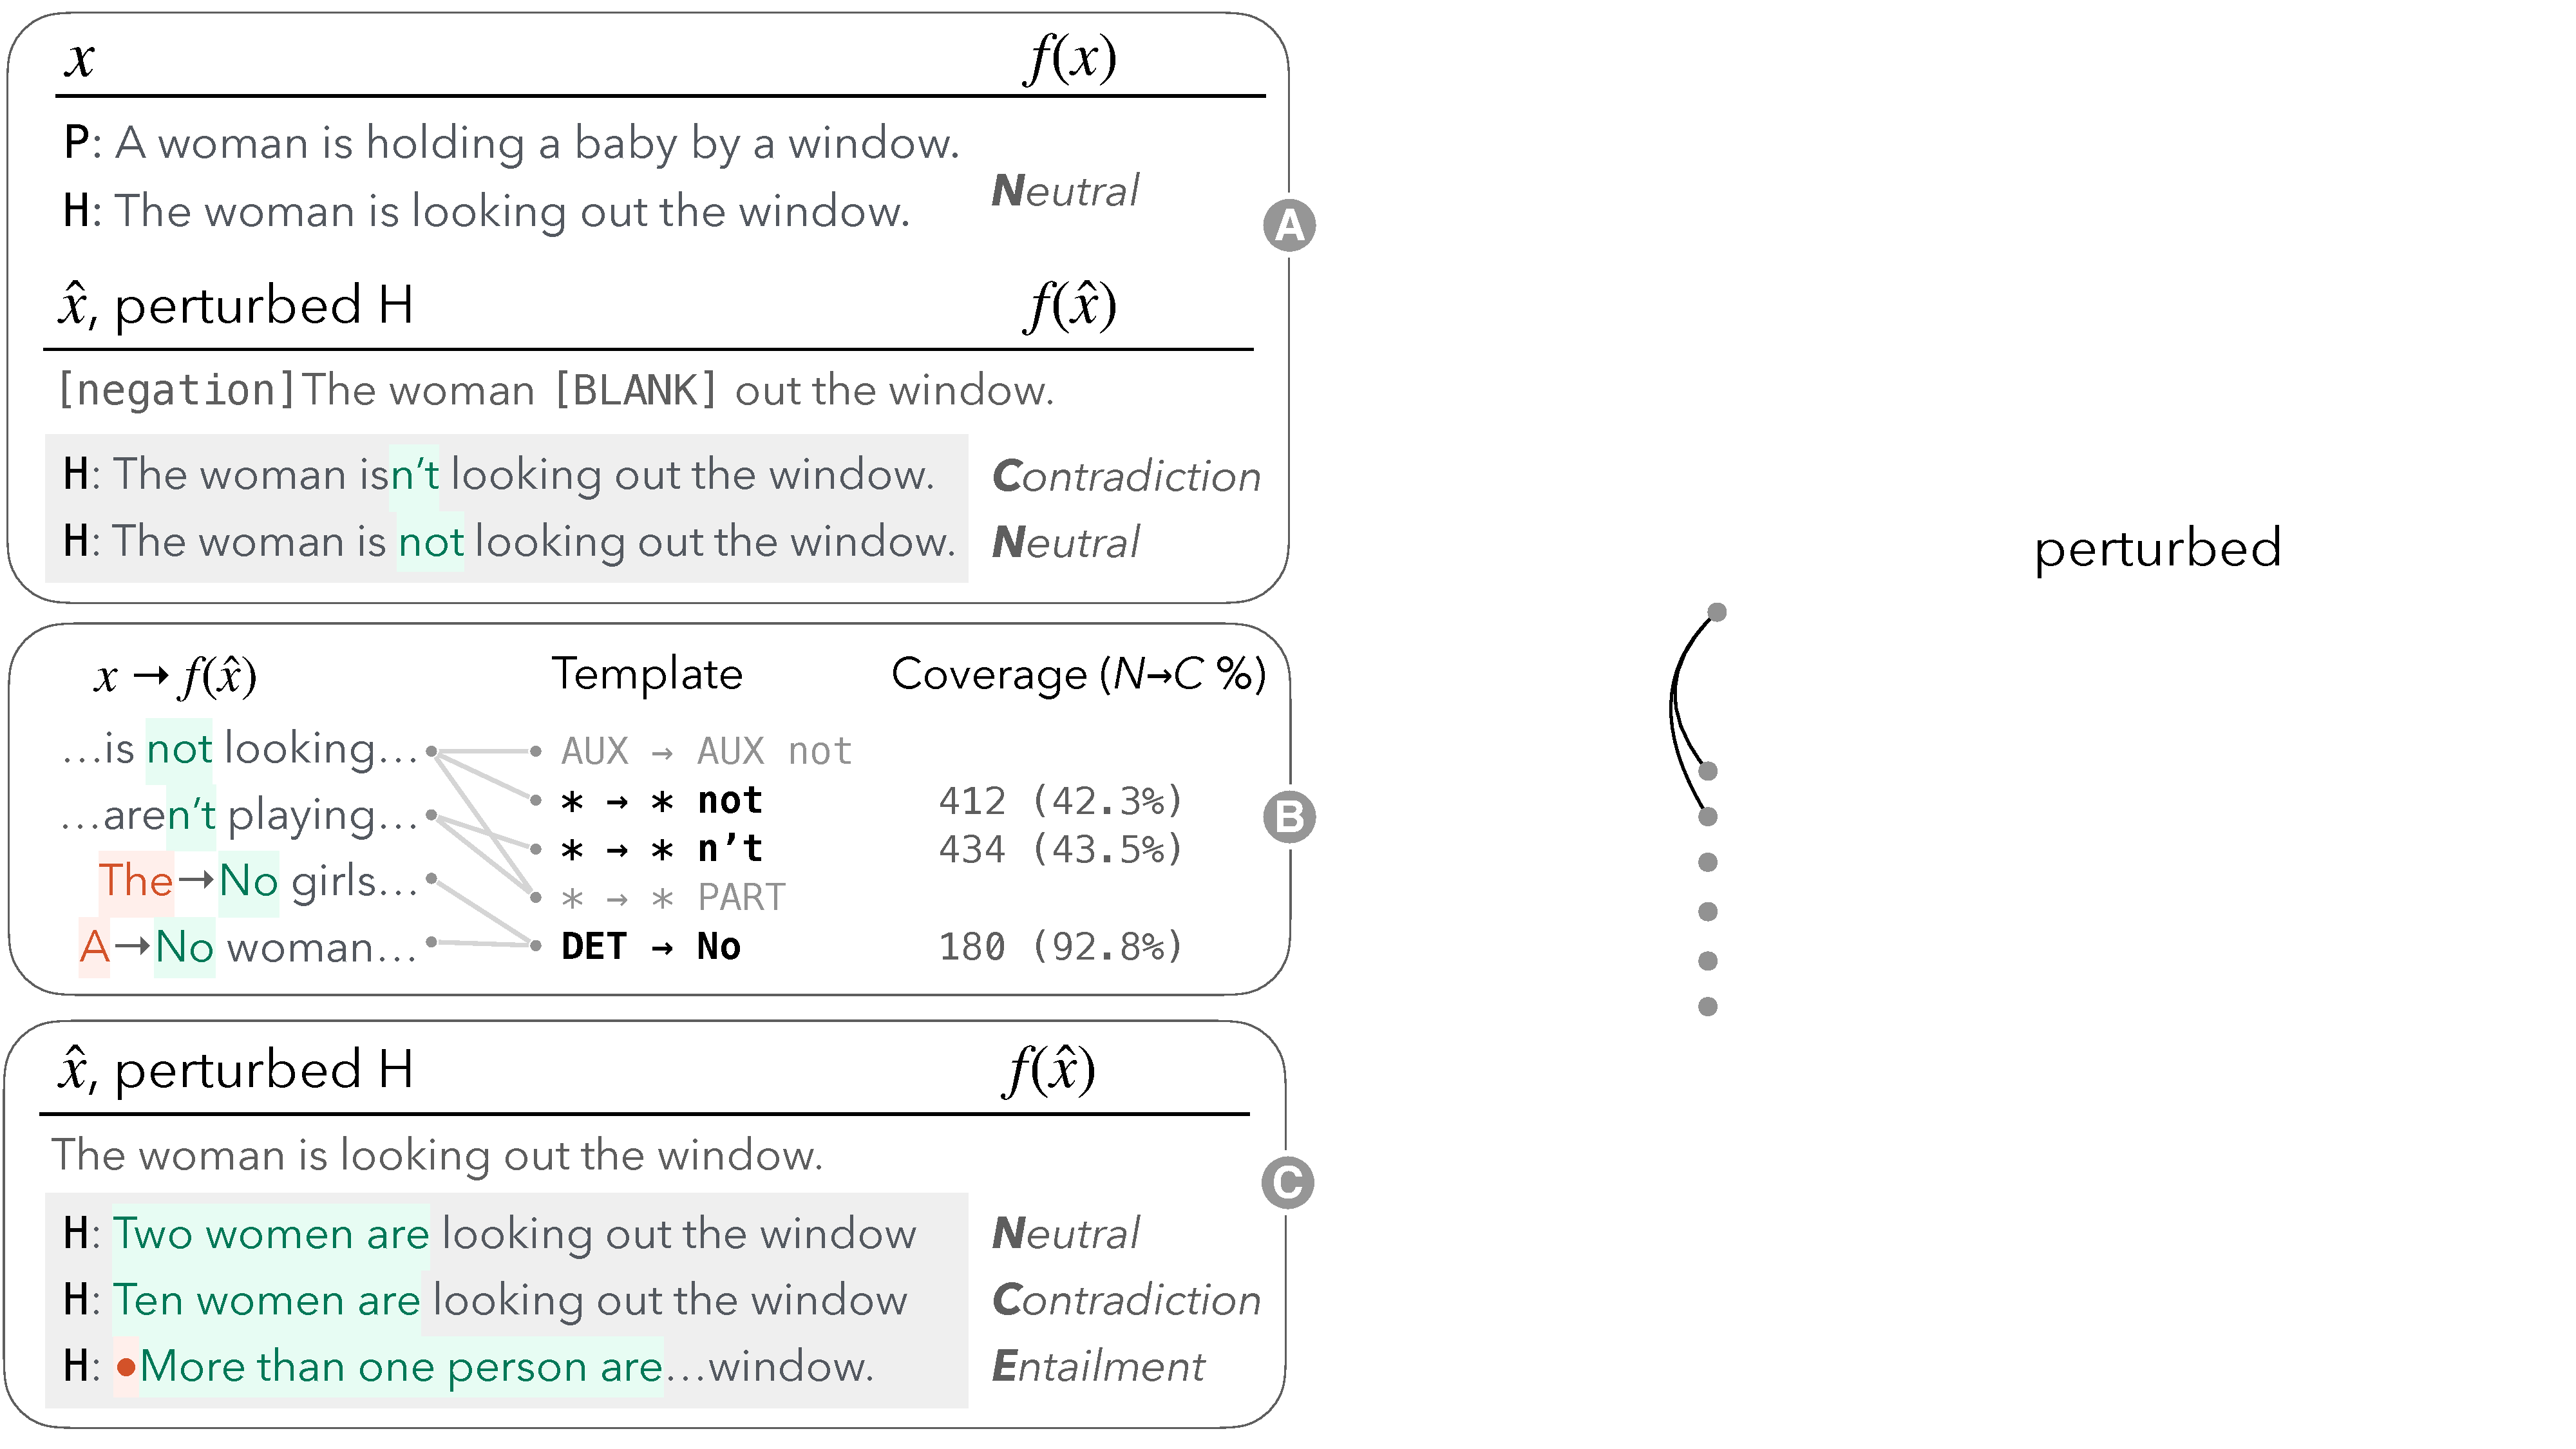
\includegraphics[trim={0.5cm 1.8cm 32.5cm 25.5cm},clip,width=1\columnwidth]{figures/err_analysis.pdf}
\vspace{-15pt}
\caption{
Another blank placement of $x$ in Figure~\ref{fig:err_analysis}A. 
Similar changes result in different predictions (should all be \uline{\emph{Neutral}}), which leads to analyses of \emph{quantifiers}.
}
\vspace{-10pt}
\label{fig:err_analysis_quantifier}
\end{figure}


\emph{Drill-down through interactive blanking.}
If \add{not} and \add{n't} are generally stable, what causes the difference in Figure~\ref{fig:err_analysis}A?
We can drill down by adding blanks to the negated hypotheses.
For example, inspired by the returns from \exinline{\texttt{[BLANK]} is\add{n't}/\add{not} looking out the window}, we find changing \remove{woman} to \add{girl}, \add{boy}, and \add{man} in both the \emph{P} and the \emph{H} would all eliminate the \add{n't}/\add{not} difference, whereas \add{person} cannot.
Intrigued by the impact of subjects, we also apply a similar blanking to the original \emph{H}.
%: \exinline{\texttt{[BLANK]} looking out the window.}
%When the fillin is \add{two women are}, the prediction is neutral, but it flips to contradiction when the number is \add{ten}.
%When we instead use the fill in \add{more than one person is}, the model instead returns entailment.
The wild predictions in Figure~\ref{fig:err_analysis_quantifier} lead us to further hypothesize that the model does not understand quantifiers, which we verify in Appendix~\ref{appendix:err_analysis_quantifier_case}.


\paragraph{Takeaways.}
\sysname provides unique support for interactive and targeted generation.
First, \emph{over-}generation helps analysts contrast similar perturbations and form hypotheses that might otherwise be missed.
Analysts rarely check both \swap{is}{is not} and \swap{is}{isn't}, and therefore can overlook potential differences, echoing our observation (\S\ref{sec:app_explain}) that manual counterfactual analysis can be misleading.
Using \tagstrs, \sysname also reveals patterns that are hard to retrieve from existing masked language models.
When applying RoBERTa to the same blanked (masked) hypotheses, we obtain less than 5\% negation counterfactuals compared to \sysname.
Instead, over 1,000 counterfactuals concern \swap{is}{\texttt{VERB}} and \swap{are}{\texttt{VERB}}.
Similarly, RoBERTa can not produce the examples in Figure~\ref{fig:err_analysis_quantifier}, as it focuses on single word replacement.
%The apparent gap highlights \sysname's support on interactive and targeted generation.

%Moreover, with \sysname diversifying the text chunks to change, it \sysname helps contrast similar changes that happen at different places.
%While \sysname enables the comparison between \swap{\texttt{VERB}}{\texttt{not VERB}} and \swap{\texttt{DET}}{no}, RoBERTa focus on changing \texttt{VERB}: the top two templates from it are \texttt{\swap{is}{VERB}} and \texttt{\swap{are}{VERB}}, producing 1000 conterfactuals in total.